\documentclass[conference]{IEEEtran}
\usepackage{graphicx}
\usepackage{amsmath}
\usepackage{amssymb}
\usepackage{xcolor}
\usepackage{url}
\usepackage[ruled]{algorithm2e}
\usepackage{algorithmic}
\newtheorem{lemma}{Lemma}
\newtheorem{theorem}{Theorem}
\newtheorem{property}{Property}
\newtheorem{corollary}{Corollary}
\newtheorem{definition}{Definition}[section]
\newtheorem{example}{Example}[section]

\title{ An automata theoretic framework for analyzing effects
of code replacement attacks on scheduling}
\begin{document}

\maketitle
\begin{abstract}
Industrial Control Systems (ICS) used in manufacturing, power generators
and other critical infrastructure monitoring and control are  ripe targets for cyber attacks
these days. Examples of such attacks are abundant such as attacks on Iranian nuclear enrichment plant with Stuxnet in 2009,
on German steel plant in 2014, Ukrainian power system in 2015 and 2016.
 Usually in ICS, multiple control loops work concurrently and share various resources including the
communication bus through which they interact with sensors and actuators. Real-time scheduling of concurrent control applications while competing for shared 
resources demands a delicate balance between performance and real-time constraints.
A possible insider attack could be the replacement of a previously vetted control application 
or other components in the system,
during a system update.  In this paper, we
propose an automated framework that addresses the effect of such replacement attacks from the perspective of loss of control
performance. Given a set of control components, a control
objective to be satisfied by the control ensemble, the question
of schedulability and synthesis of a scheduler that can ensure
the desired control performance has been recently studied in literature. In this paper, we extend this idea further to 
build an automata theoretic framework for assessment of replacement attacks on schedulability. We have built an end-to-end framework that takes in a set of control components,
their variants (after replacement), a control objective
to be guaranteed, and performs an automated schedulability
assessment. We report some preliminary experiments of our
framework on simple benchmarks.

\end{abstract}

%\begin{IEEEkeywords}
% CyberPhysical System, \textcolor{black}{Cooperative Control}, \textcolor{black}{Code Replacement Attack}, 
% \textcolor{black}{Insider threat},  $\omega$-regular language, B\"{u}chi Automaton, Schedulability
%\end{IEEEkeywords}
\section{Introduction} \label{sec:intro}
\noindent
Most critical infrastructures such as power grid, sewage control, power generation plants, industrial automation etc., are cyber-physical systems. Cyber-Physical systems have the following major interacting constituents -- a set of control components with physical dynamics governed by laws of physics, modeled with partial differential equations, and another control scheduling component, which co-ordinates control of the physical dynamics and schedules them for execution. For very large and geographically distributed cyber physical systems, the control trajectory is designed to be stable and reliable with very complex distributed as well as centralized control. The control components today 
routinely involve a non-trivial amount of software, running on embedded control units on-board, to support and run any moderately sophisticated CPS infrastructure. \\

\noindent
In recent history, cyber physical systems have been a popular victim of choice for so called cyber attacks, the effects of which have been moderate to as ravaging as blackouts~\cite{blackout} or financial loss. This has prompted 
NIST~\cite{nist} to promote cyber security frameworks for critical infrastructure~\cite{cs-Framewrok} as 
one of the themes of immediate research attention. Given that no cyber security framework is full proof, significant research thrust is being invested in recent times to develop techniques that allow us to continually monitor the physical dynamics of these systems and look for any anomalies that could be indicative of cyber attack induced problems. Early detection of system dynamics changes would allow us to contain the damage by immediately islanding parts of the system which point to possible origin areas in the infrastructure. \\

\noindent
Research in security of CPS is 
extremely crucial for developing technologies for cyber attack detection, prevention, and countermeasures. \textcolor{black} {Systematic} studies on different sources of cyber attacks have revealed myriads of possibilities by which these cyber threats can 
propagate inside a CPS infrastructure. 
%A popular and widely acknowledged means of cyber-attack, {\em phishing attacks}, originate when someone whose desktop
%is connected to the control network opens an email containing a payload, which can then
%take over the control of the business network, and in turn the control network. However, since
%much of the cyber threat models also assume insider knowledge or sabotage, even an isolated
%control network is not devoid of cyber-attack possibilities. A popular example  is the notorious Sony Pictures hack~\cite{SonyHack2014} which leaked a release of confidential data from the film studio Sony Pictures. 
A person with local or remote access
to the equipment of the physical plant, or access to the various interfaces such as programmable
logic controllers (PLCs) or other Intelligent Electronic Device (IEDs) that are connected to the
physical system for measurement and control, can exploit a vulnerability in these devices to
induce an attack on the system. One could also gain access to the control network, and create
various kinds of man-in-the-middle attacks by either suppressing measurements or control
actuation signals, replaying stale measurements or actuation signals, or even injecting
maliciously planned false data. These kinds of attacks would then mislead the controllers, and
wrong control actions could lead to disastrous industrial accidents. One could also hack into the
controllers or the various other computing elements in the control center such as the process control servers by
exploiting vulnerabilities in their design and attack the cyber physical system. In fact, in
case of the Stuxnet worm~\cite{stuxnet}, \textcolor{black} {vulnerabilities} in the Siemens SCADA system were exploited. Individual areas of cyber security research have received
much recent attention in academia, e.g. cryptography; crypto-analysis; network
security in the form of firewall and other perimeter security techniques, and intrusion detection, anti-virus software, and static analysis of software to detect vulnerabilities and zero-day attacks;
hardware Trojan detection. \\ 

\noindent
{\bf Problem addressed in this paper:} This paper studies the CPS security problem from a different perspective: the focus of study in this paper is {\em schedulability attacks}, wherein some or parts of a control component are compromised, and the scheduler is unable to schedule the different components in any way to meet the control objectives of the CPS.  In an industrial control environment with real time control components, this can lead to disaster since some of the components may malfunction due to lack of input from the scheduler. As an example, slowing down a
particular process in industrial manufacturing can cascade a chain of failures in the whole
assembly line. In this paper, we propose an idea that will demonstrate that such
attacks for real-time SCADA systems can be guarded against by statically analyzing the
legitimate control programs, and constructing an omega-regular language based timing signature,
which can then be periodically checked on the running components to check for schedulability. The idea presented here is based on the timing signature analysis for omega-regular languages~\cite{WeissFAA09}, in the context of real-time communication scheduling in CPS. \\

\noindent
{\bf Contributions of this work:}
In this paper, we address the problem of detecting schedulability attacks. Given a set of control components, a control objective 
to be satisfied by the control ensemble, the question of schedulability and 
synthesis of a scheduler that can ensure the desired control performance has been recently studied in literature~\cite{WeissFAA09},\cite{AlurW08},~\cite{GhoshMDHD16}. 
In this paper, we extend the same philosophy to build an automata theoretic framework for assessment of replacement attacks on schedulability. The foundation of our attack analysis framework is based on the notion of infinite automata-based reasoning of control performance and schedulability analysis, as illustrated in the following section. Automata theoretic modeling frameworks have been quite popular in literature for a wide variety of applications. Additionally, the power of finite automata over infinite words (B\"{u}chi automata in particular) have been exploited in recent literature in control performance and stability analysis. Our work is another step in the same direction for assessing the effect of schedulability attacks in cyber-physical control. \\


\noindent
{\bf Organization:} This paper is organized as follows. Section~\ref{sec2} presents related work. Section ~\ref{sec3} describes the problem definition for this work along with a motivating example. Section~\ref{sec4} presents the solution architecture. Section~\ref{sec5} presents an overview of the tool we have developed. Section~\ref{sec7} concludes this discussion.


%\section{Related Work} \label{sec2}
Replacement attacks \cite{GhoshHD12} carried out by internal employees, phishing attacks, code injection attacks have been known to be a vector for cyber-attacks for a while. Stuxnet analysis showed that such
attacks were part of the repertoire in that case.  The work in \cite{DBLP:conf/acns/MingXLW0M15} %\cite{DBLP:journals/virology/MingXLWLM17} 
describe the idea of replacement attack on malware behaviour. Malware belonging to
same family are supposed to show similar behaviour but 
  if the replacement  attack changes the behaviour specification, then inspite of being from same family, their behaviour will be different. Malware
  interact with operating system through system call. A system call dependency graph(SCDG) shows the data flow dependency among system call. In this paper,
  they propose the idea of SCDG replacement and the after replacement effect on the malware behaviour. To detect the attack, malware analysts are required 
  to put extra efforts to re-analyse the similar samples. Further,  \cite{DBLP:conf/vee/GhoshHD12} represents how the protected PVMs(Process-level virtual machines) can be replaced with attack VM(virtual
  machines) which makes the application more vulnerable to analysis and modification. The analysis of  replacement attck on generic watermarking system described in \cite{DBLP:conf/ccs/KirovskiP02}. 

The idea of automata based control scheduling has been discussed in \cite{WeissA07}. They express
the communication interface among the control components using a formal language. This work illustrates how the interfaces of discrete-time switched linear systems
can be expressed using a B\"{u}chi automaton. Authors in \cite{AlurW08}  describe CPU scheduling
in terms of finite machines over infinite words. The infinite words depict the particular time 
slot for which a particular resource can be allotted to a specific control component. The work in \cite{WeissFAA09} applies automata based scheduling on networks, to formalize the effect of bus scheduling and network stability. Further, \cite{GhoshMDHD16} describes how the interfacing among 
the control actions can be modeled by B\"{u}chi automata to guarantee stable and reliable
scheduling. This work presents a methodology for construction of a scheduler automata 
where each state represents one particular control schedule while generating the permissible 
schedule in terms of a $\omega$-regular language. Our work is an application framework based on the contributions above, with specific focus to component replacement attacks and schedulability analysis. While one of the major control objectives discussed in the above contributions has been exponential stability, which we assume to be satisfied for individual control components, we propose to use a fairness schedule in our work, that requires a different modeling strategy, as explained in the following. More importantly, our work here can be considered as an end-to-end framework on automata-based control performance modeling and assessment. \\
  
 
  

%\input{background}
\section{Problem Model and Motivating Example} \label{sec3}
\noindent
To explain our problem, we consider a control application system consisting of an ensemble of concurrently active control applications / loops. Each control application is partitioned into a set of
tasks. The control tasks communicate via a shared bus. The messages on the shared bus are also scheduled using a given arbitration policy. When a control loop executes, it carries out the set of tasks as specified by different states in its control state machine. Among all these states, some
states require bus access, for which the control loop presents a request to the bus arbiter. These requests are considered by the bus arbiter / scheduler which decides on a bus scheduling strategy to grant bus access to the different control loops over time at different time slots. \\

\noindent
As discussed in recent literature, we consider each participating control application is modeled as a B\"{u}chi automaton. B\"{u}chi automatons~\cite{leeuwen90/Thomas90} have been a popular mechanism of choice for modeling applications that require finite automatons over infinite strings or words. The basic structure of such automatons is similar to their finite counterparts, with the exception of the acceptance conditions, as described below.
A B\"{u}chi automaton is described as a five tuple, 
$A = (Q,I,\delta,q_0,F)$, where $Q$ is a finite set of states, $I$ is the input alphabet, $\delta : Q$ x $I \rightarrow Q $ is the transition function, $q_0$ 
is an initial state ($q_0 \in Q$) and $F$ is a set of final states that help us model the infinitary acceptance condition. An infinite word $\lambda \in I ^ \omega$ over the input alphabet takes the automaton through an infinite sequence of states $ q_0, q_1, q_2, ....$, which describes a run of
the automaton such that $ q_{k+1} \in \delta(q_k, \delta_k)$ where $k \in \mathbb{N}$ and $\delta_k$ refers to the $k^{th}$ symbol on the input 
word $\delta$. An infinite word is accepted if some 
accepting state $q_f \in F $ appears in the run $ q_0, q_1, q_2, ....$ 
infinitely often. If 
$|\delta(q,i)| = 1$ where $ q \in Q $ and $i \in I$, then it is a deterministic 
B\"{u}chi automaton, otherwise it is non-deterministic. \\

\noindent
Each control loop is designed with a control objective in view, and the overall functioning of the system is dependent on the individual control loops meeting control objectives, along with a strategy for co-operative control of the shared message bus through which the control loops communicate with each other. We consider one such control system functioning correctly if both the above conditions are met. Meeting control objectives has been addressed in several recent articles, and is therefore, not discussed here. In contrast, we focus more on the schedulability aspect, as described below. 

\subsection{Schedulability and code replacement attack:} 
\noindent
We now characterize the schedulability requirement below. 
A set of concurrent control loops, each expressed as a B\"{u}chi automaton, is considered {\em schedulable} if there exists a strategy to schedule the individual control loops on the shared bus {\em infinitely often}.
The scheduling objective is defined in the lines of infinitary acceptance, as is the case with B\"{u}chi objectives. Intuitively, a scheduler should be able to allocate bus access to each individual control loop infinitely often. More specifically, given any infinite run of the composed system, at least one constituent task (i.e. bus accessing / accepting state) from each control loop should repeat infinitely often. We consider the system {\em safe} if this holds, {\em attacked} otherwise. We conclude that a {\em code replacement attack} has been carried out if a system,  initially safe and schedulable, turns out to be non-schedulable. 

\begin{figure}
\begin{center}
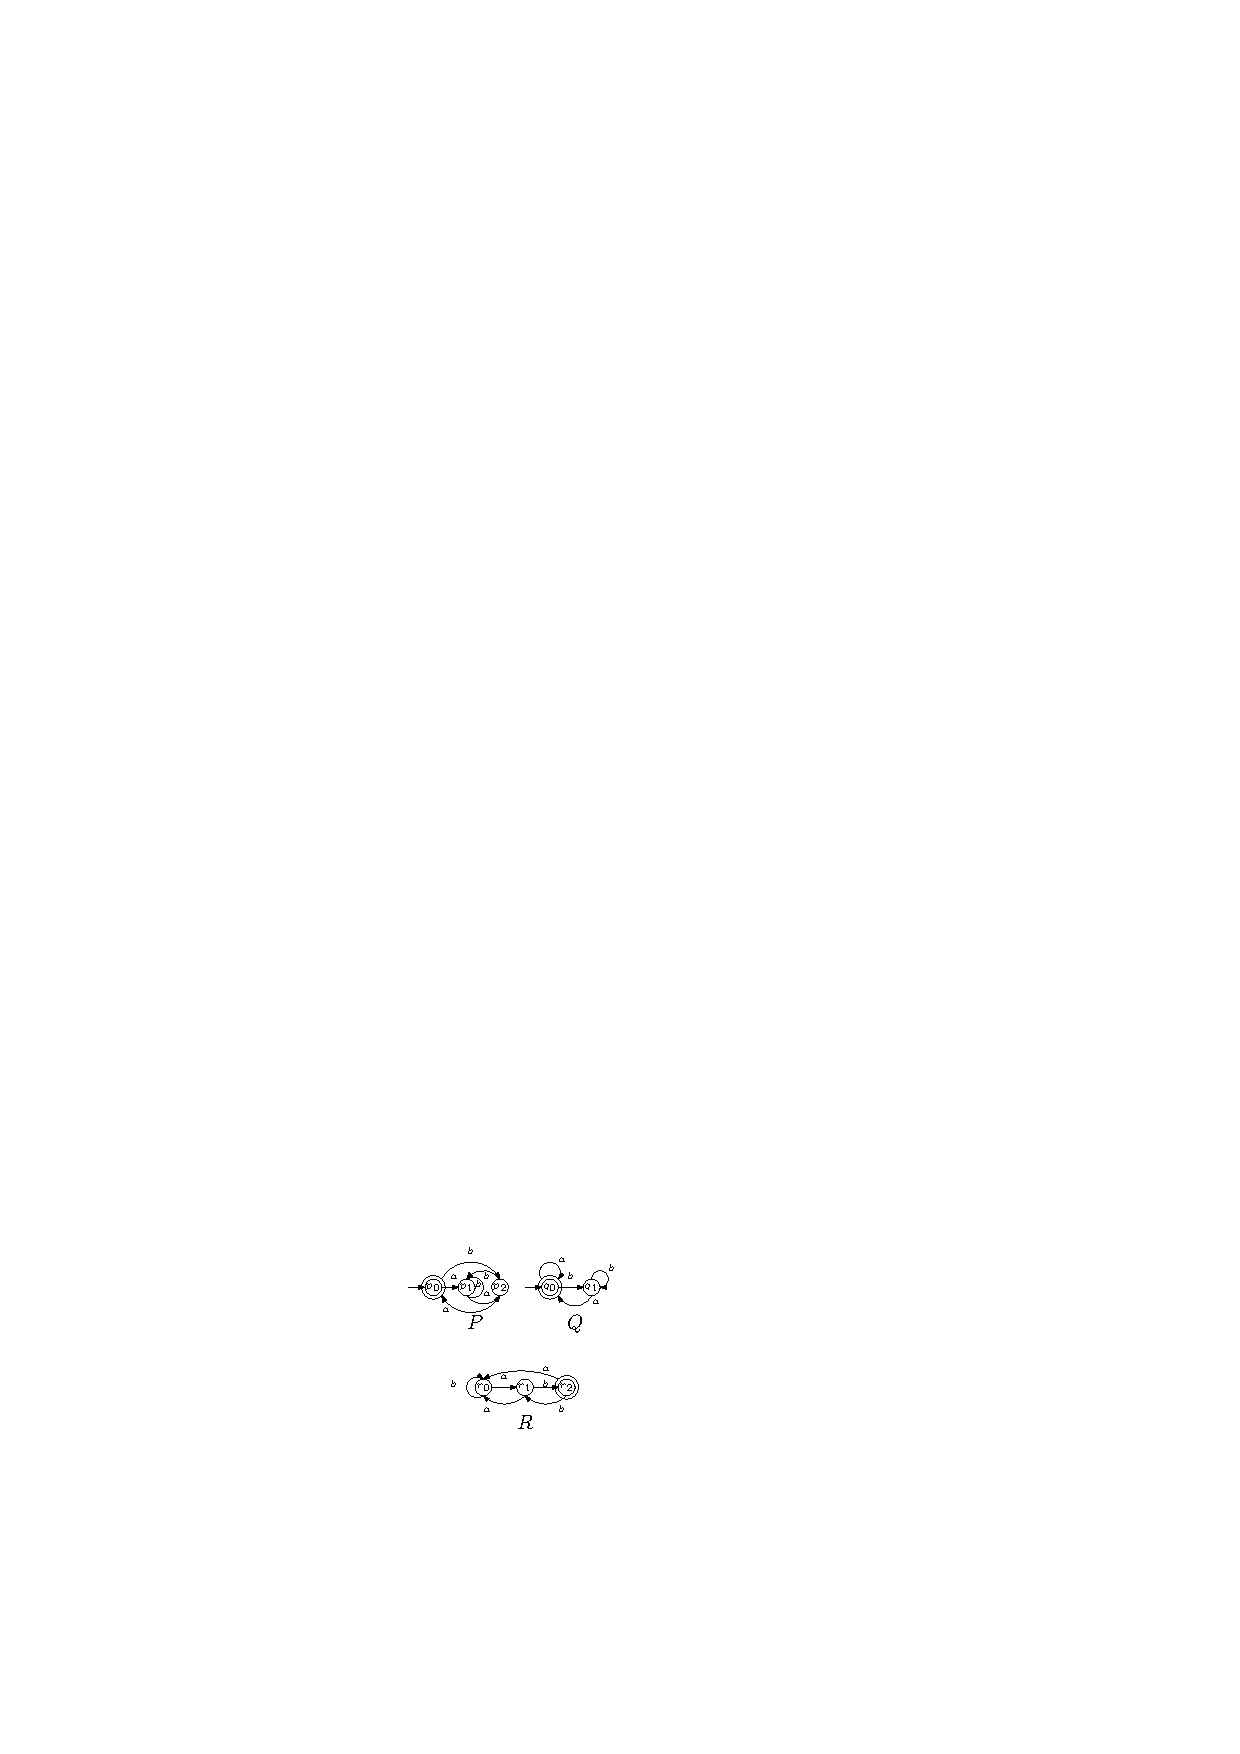
\includegraphics[width=50mm]{original.pdf}
\end{center}
%\vspace{-0.1in}
\caption{{\em Initial Control loops}}
\label{state}
\end{figure}

\subsection{Motivating Example:}
\noindent
We explain our problem statement with a small example. Fig\ref{state} presents three automatons $P,Q$ and $R$ representing three different control applications.
Each has one initial state and an acceptance state. The acceptance states are the bus accessing states
of the automaton. To check for schedulability, we first construct the concurrent composition (the intersection automaton) of the individual automatons, as shown in Fig \ref{state-transition}. The product construction is a little different from the classical product of finite automatons, and will be explained in the following section. \\ 

\noindent
We now consider a code replacement attack take places on this system. The resulting automaton is depicted in Fig \ref{replaced}.
As a result of this attack, one of the control loops is changed, as a result of which, there is a change in the structure of the intersection automaton. Our schedulability assessment on the new product automaton fails. As we can see in Fig \ref{graph_replaced}, there are no cycles which satisfy our infinitary scheduling condition, thus schedulability is no longer guaranteed and we conclude that a code replacement attack has taken place.

\begin{figure}
\begin{center}
\includegraphics[width= 75mm]{graph.eps}
\end{center}
%\vspace{-0.1in}
\caption{{\em Initial Intersection automaton}}
\label{state-transition}
\end{figure}

\begin{figure}
\begin{center}
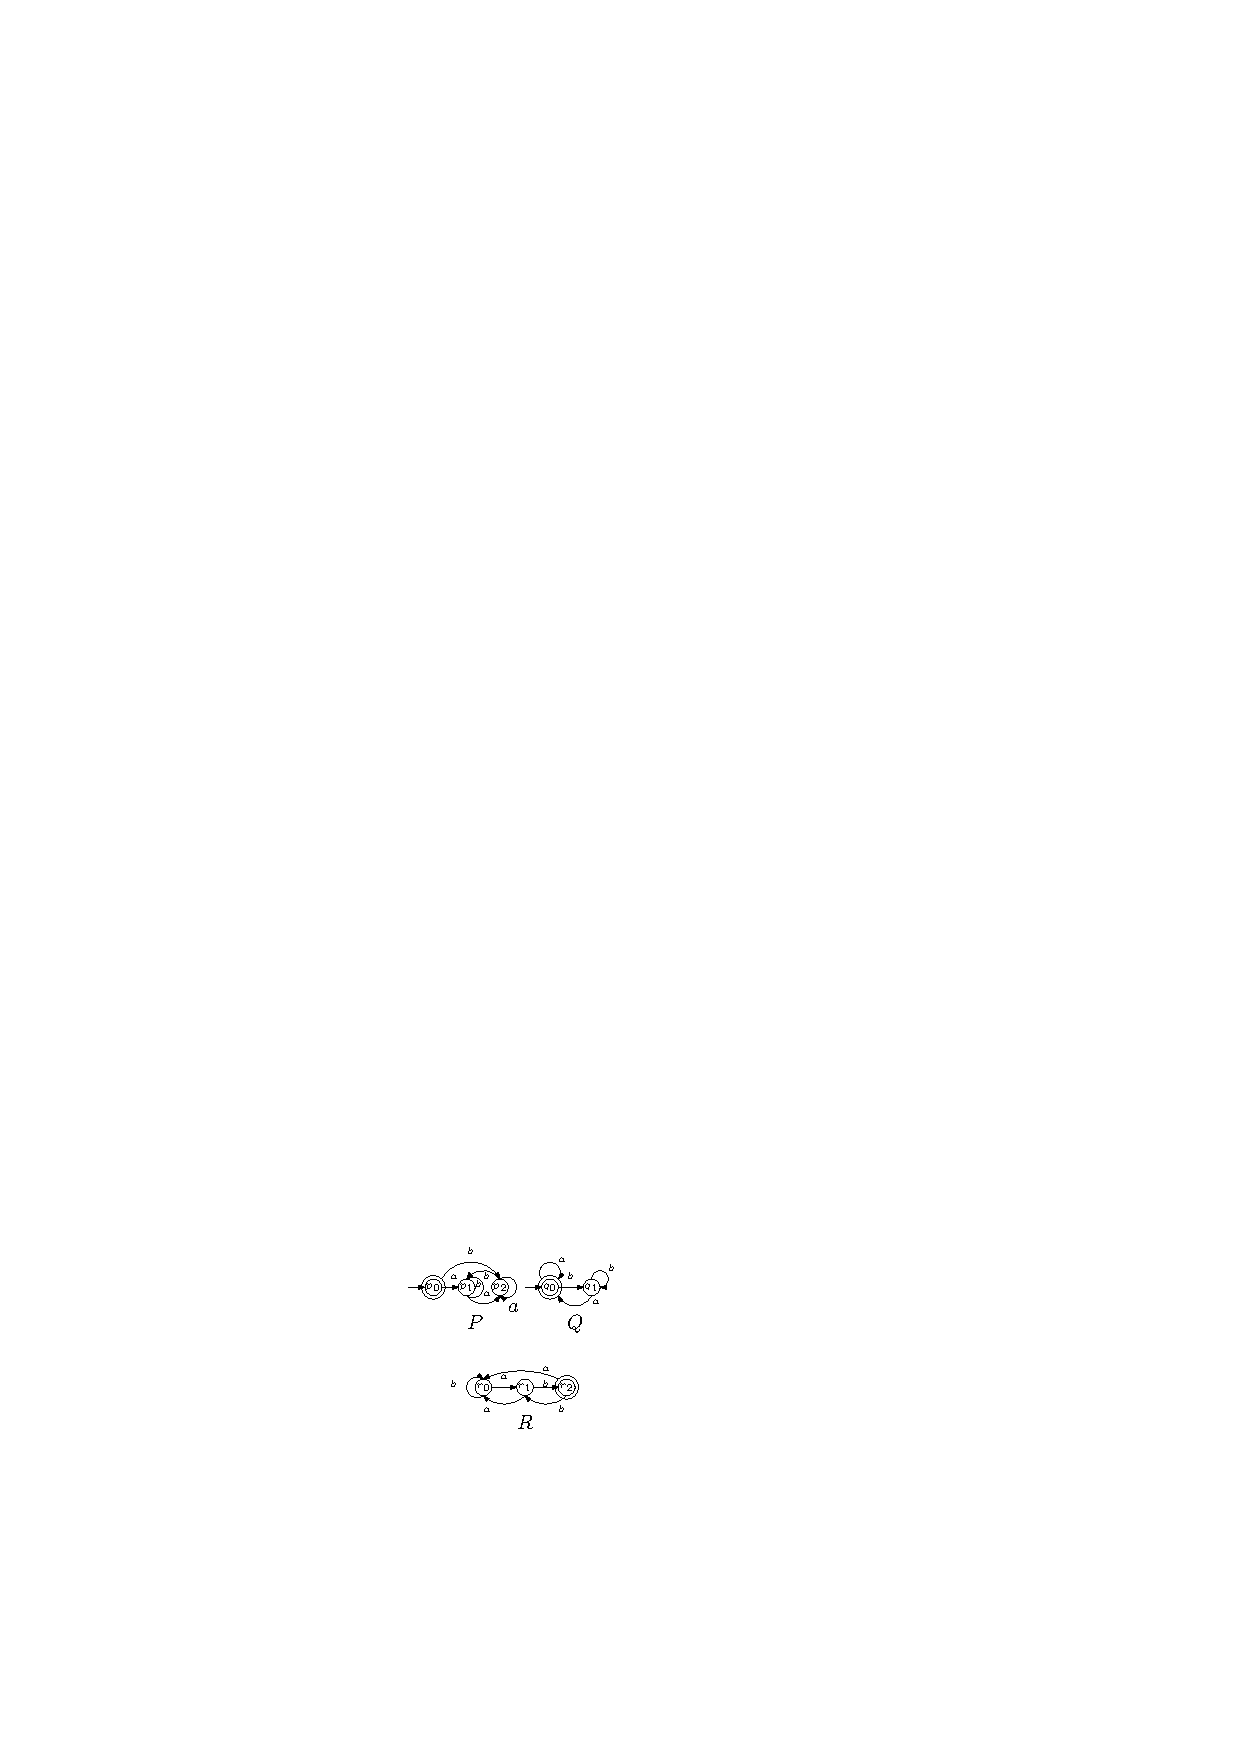
\includegraphics[width= 50mm]{replaced.pdf}
\end{center}
%\vspace{-0.1in}
\caption{{\em Modified control loops after a replacement attack}}
\label{replaced}
\end{figure}


\begin{figure}
\begin{center}
\includegraphics[width= 50mm]{graph_replaced.eps}
\end{center}
%\vspace{-0.1in}
\caption{{\em Intersection automaton after a code replacement attack}}
\label{graph_replaced}
\end{figure}


%\section{Problem Model and Motivating Example} \label{sec3}
\noindent
To explain our problem, we consider a control application system consisting of an ensemble of concurrently active control applications / loops. Each control application is partitioned into a set of
tasks. The control tasks communicate via a shared bus. The messages on the shared bus are also scheduled using a given arbitration policy. When a control loop executes, it carries out the set of tasks as specified by different states in its control state machine. Among all these states, some
states require bus access, for which the control loop presents a request to the bus arbiter. These requests are considered by the bus arbiter / scheduler which decides on a bus scheduling strategy to grant bus access to the different control loops over time at different time slots. \\

\noindent
As discussed in recent literature, we consider each participating control application is modeled as a B\"{u}chi automaton. B\"{u}chi automatons~\cite{leeuwen90/Thomas90} have been a popular mechanism of choice for modeling applications that require finite automatons over infinite strings or words. The basic structure of such automatons is similar to their finite counterparts, with the exception of the acceptance conditions, as described below.
A B\"{u}chi automaton is described as a five tuple, 
$A = (Q,I,\delta,q_0,F)$, where $Q$ is a finite set of states, $I$ is the input alphabet, $\delta : Q$ x $I \rightarrow Q $ is the transition function, $q_0$ 
is an initial state ($q_0 \in Q$) and $F$ is a set of final states that help us model the infinitary acceptance condition. An infinite word $\lambda \in I ^ \omega$ over the input alphabet takes the automaton through an infinite sequence of states $ q_0, q_1, q_2, ....$, which describes a run of
the automaton such that $ q_{k+1} \in \delta(q_k, \delta_k)$ where $k \in \mathbb{N}$ and $\delta_k$ refers to the $k^{th}$ symbol on the input 
word $\delta$. An infinite word is accepted if some 
accepting state $q_f \in F $ appears in the run $ q_0, q_1, q_2, ....$ 
infinitely often. If 
$|\delta(q,i)| = 1$ where $ q \in Q $ and $i \in I$, then it is a deterministic 
B\"{u}chi automaton, otherwise it is non-deterministic. \\

\noindent
Each control loop is designed with a control objective in view, and the overall functioning of the system is dependent on the individual control loops meeting control objectives, along with a strategy for co-operative control of the shared message bus through which the control loops communicate with each other. We consider one such control system functioning correctly if both the above conditions are met. Meeting control objectives has been addressed in several recent articles, and is therefore, not discussed here. In contrast, we focus more on the schedulability aspect, as described below. 

\subsection{Schedulability and code replacement attack:} 
\noindent
We now characterize the schedulability requirement below. 
A set of concurrent control loops, each expressed as a B\"{u}chi automaton, is considered {\em schedulable} if there exists a strategy to schedule the individual control loops on the shared bus {\em infinitely often}.
The scheduling objective is defined in the lines of infinitary acceptance, as is the case with B\"{u}chi objectives. Intuitively, a scheduler should be able to allocate bus access to each individual control loop infinitely often. More specifically, given any infinite run of the composed system, at least one constituent task (i.e. bus accessing / accepting state) from each control loop should repeat infinitely often. We consider the system {\em safe} if this holds, {\em attacked} otherwise. We conclude that a {\em code replacement attack} has been carried out if a system,  initially safe and schedulable, turns out to be non-schedulable. 

\begin{figure}
\begin{center}
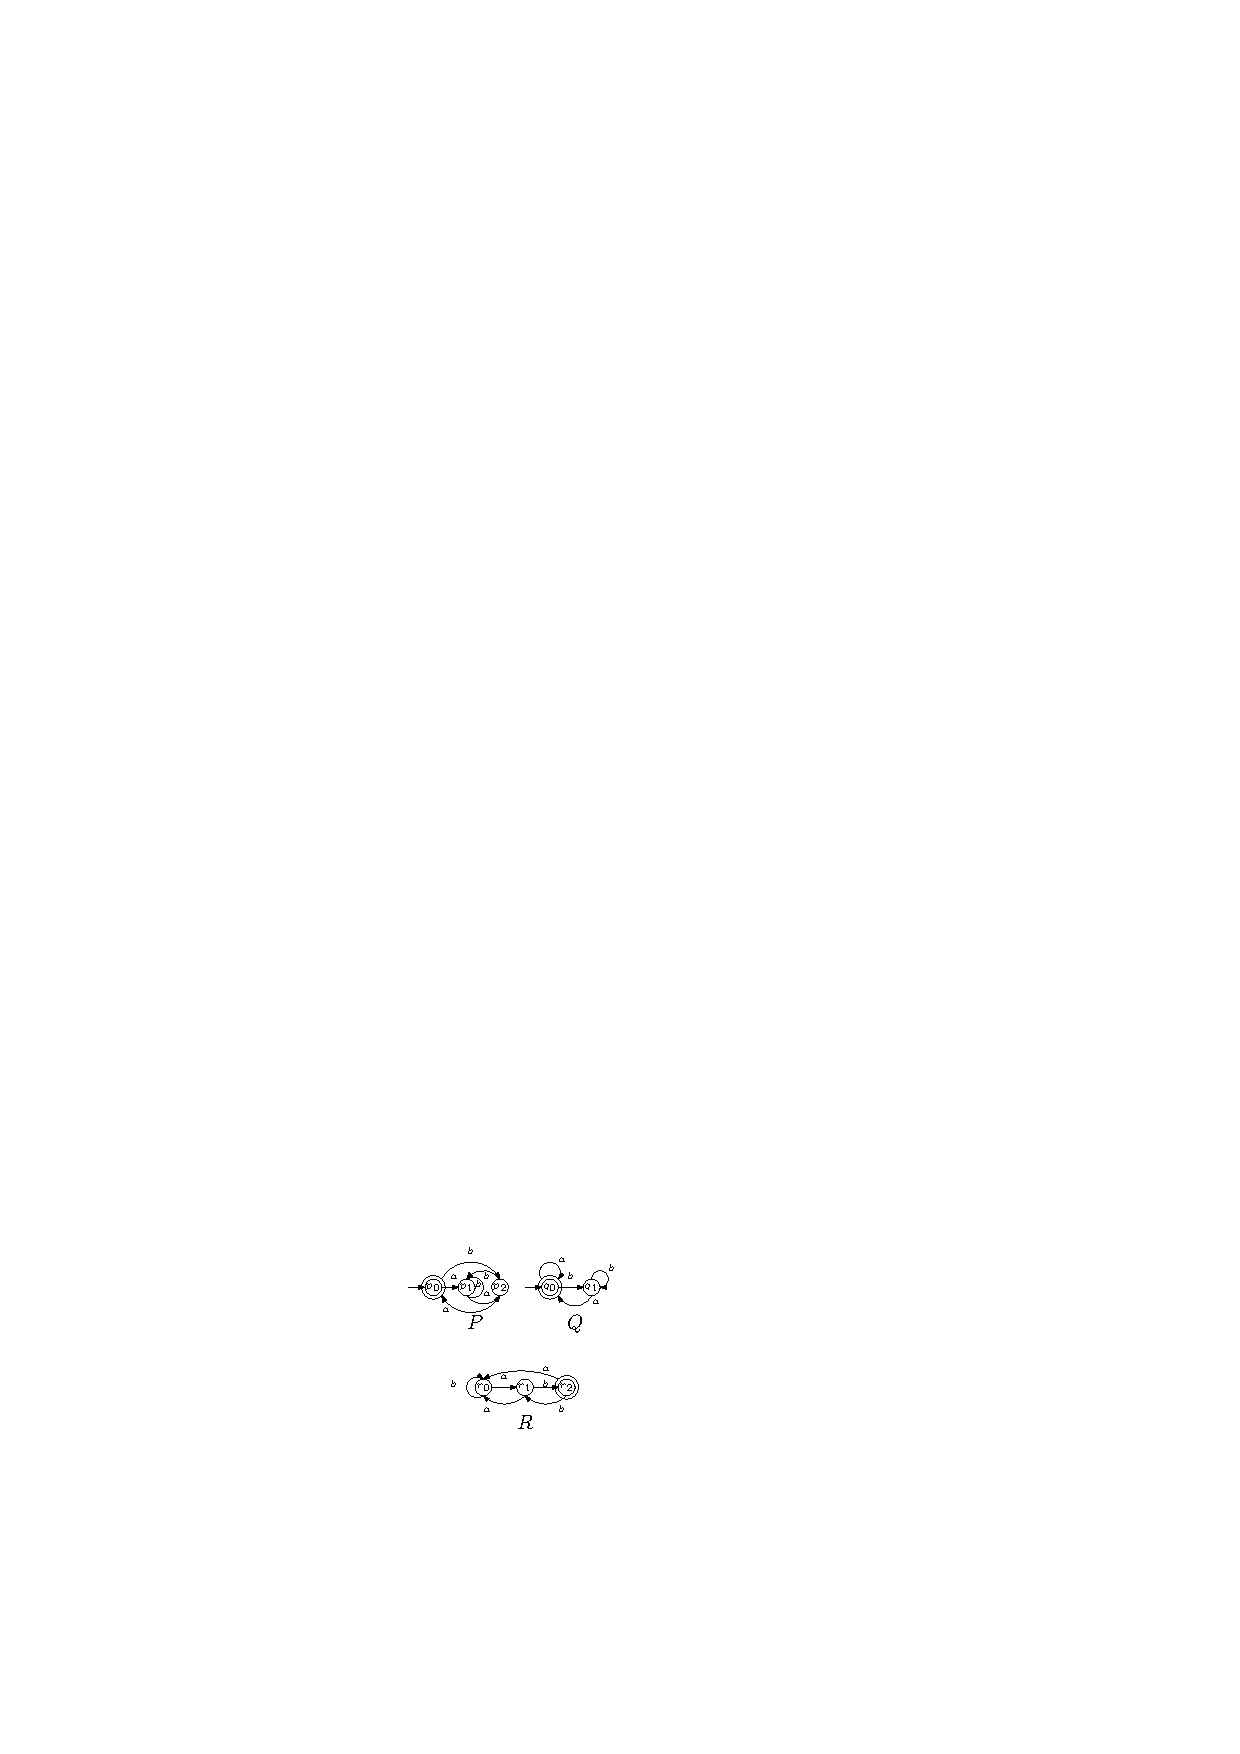
\includegraphics[width=50mm]{original.pdf}
\end{center}
%\vspace{-0.1in}
\caption{{\em Initial Control loops}}
\label{state}
\end{figure}

\subsection{Motivating Example:}
\noindent
We explain our problem statement with a small example. Fig\ref{state} presents three automatons $P,Q$ and $R$ representing three different control applications.
Each has one initial state and an acceptance state. The acceptance states are the bus accessing states
of the automaton. To check for schedulability, we first construct the concurrent composition (the intersection automaton) of the individual automatons, as shown in Fig \ref{state-transition}. The product construction is a little different from the classical product of finite automatons, and will be explained in the following section. \\ 

\noindent
We now consider a code replacement attack take places on this system. The resulting automaton is depicted in Fig \ref{replaced}.
As a result of this attack, one of the control loops is changed, as a result of which, there is a change in the structure of the intersection automaton. Our schedulability assessment on the new product automaton fails. As we can see in Fig \ref{graph_replaced}, there are no cycles which satisfy our infinitary scheduling condition, thus schedulability is no longer guaranteed and we conclude that a code replacement attack has taken place.

\begin{figure}
\begin{center}
\includegraphics[width= 75mm]{graph.eps}
\end{center}
%\vspace{-0.1in}
\caption{{\em Initial Intersection automaton}}
\label{state-transition}
\end{figure}

\begin{figure}
\begin{center}
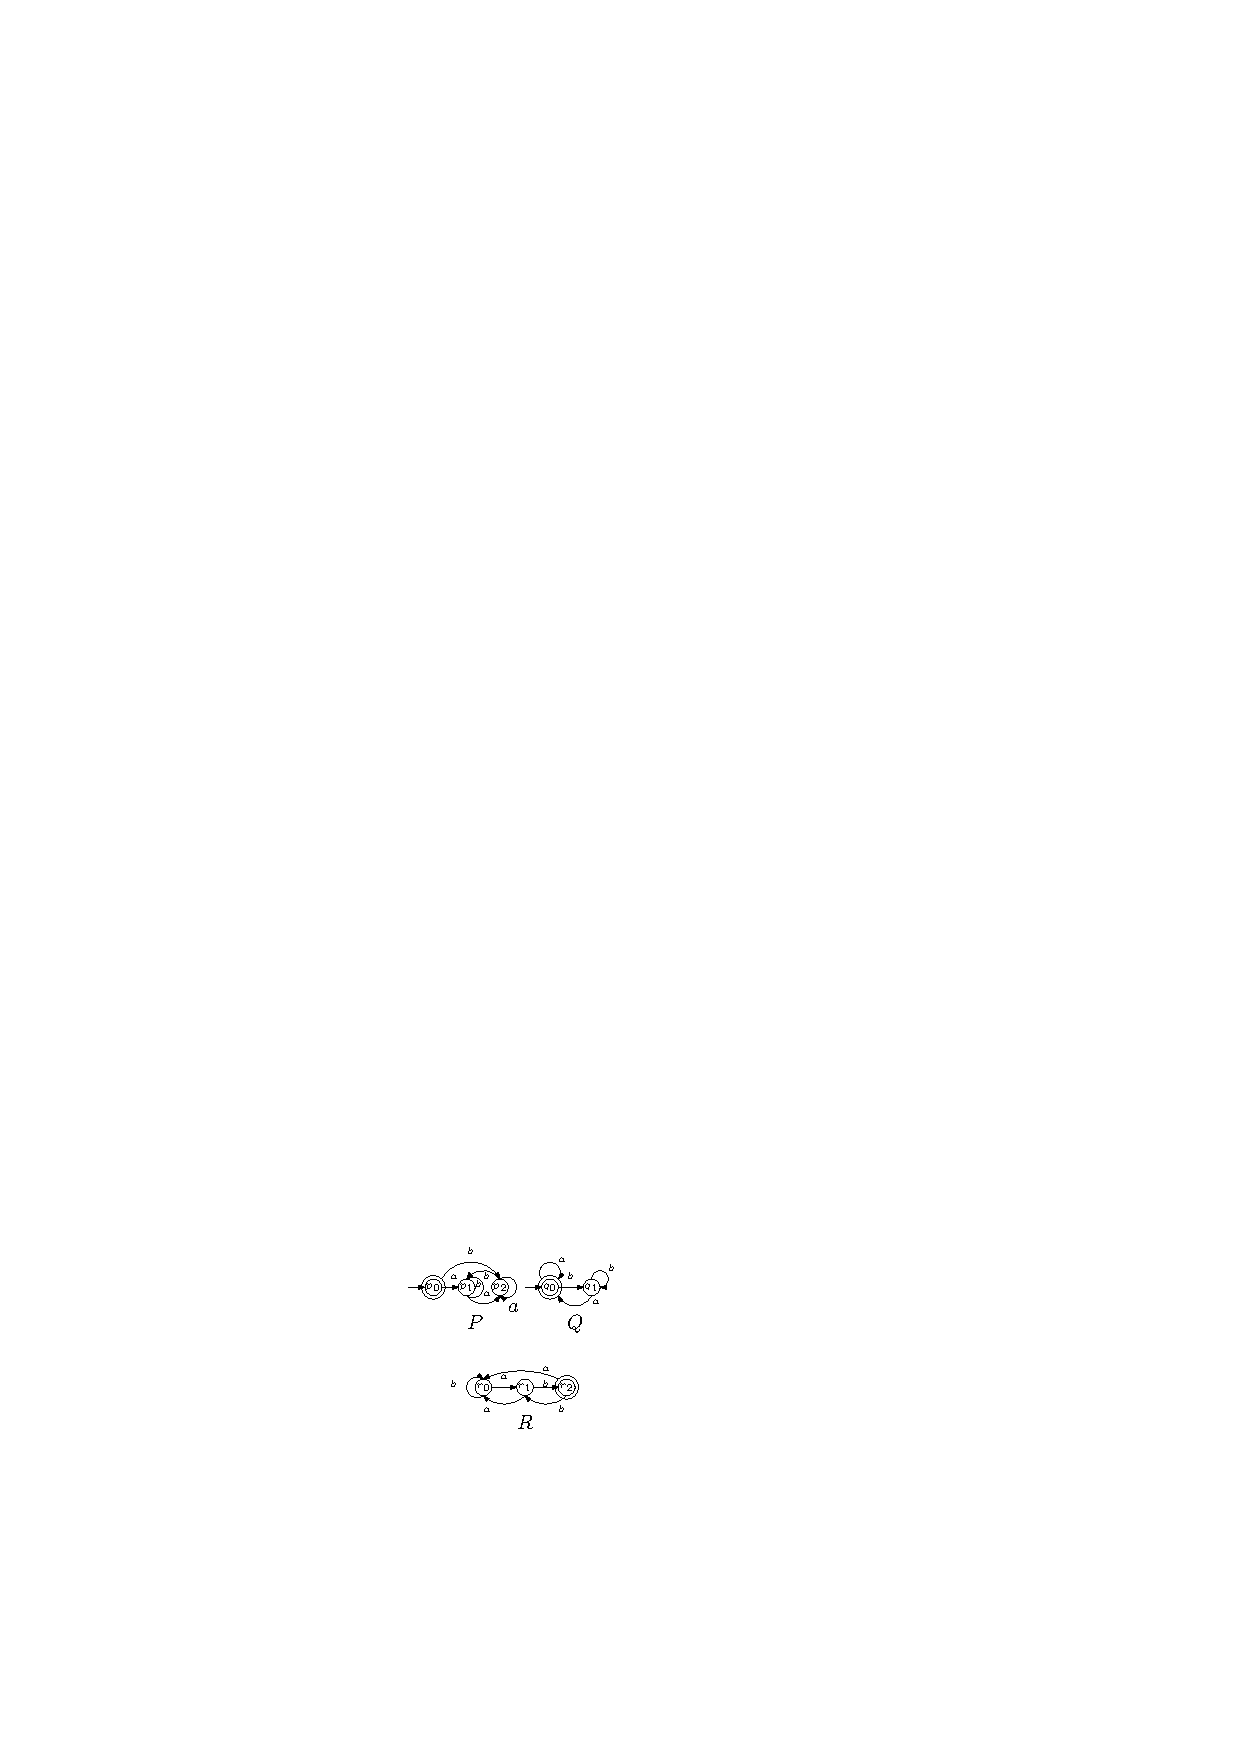
\includegraphics[width= 50mm]{replaced.pdf}
\end{center}
%\vspace{-0.1in}
\caption{{\em Modified control loops after a replacement attack}}
\label{replaced}
\end{figure}


\begin{figure}
\begin{center}
\includegraphics[width= 50mm]{graph_replaced.eps}
\end{center}
%\vspace{-0.1in}
\caption{{\em Intersection automaton after a code replacement attack}}
\label{graph_replaced}
\end{figure}


%\input{Motivating_examples}
\section{Solution Architecture} \label{sec4}
\noindent
In this section, we explain our solution architecture for schedulability assessment. As described in the previous section, we are given a set of $n$ control loops, with their bus access states marked as the accepting ones. Recall that our scheduling objective is to be able to grant bus access infinitely often to each control loop. To check if the system is safe and schedulable, we carry out the following steps: 

\begin{itemize}

\item We compute the product of the individual control loops using the construction explained below. 

\item Once the product is computed, we look for the presence of a cycle that contains at least one state from each control loop. In other words, on any infinite run of the product automaton, each control loop repeats infinitely often and is therefore, granted bus access infinitely often as well. 

\end{itemize}


\subsection{Intersection Automaton construction}
\noindent
Given a collection of control loops, each expressed as B\"{u}chi automatons, we describe below the methodology for computing their product~\cite{DBLP:books/ws/automata2012/ChevalierDMP12}, which is an important step in our work. For the sake of simplicity and ease of illustration, we explain the product construction in terms of two automatons. 
Let us consider the two B\"{u}chi automatons P and Q, as shown in Fig \ref{fig1} and defined by the
conventional five tuple:

$P = \{(p_0,p_1),(a,b),p_0, Q \times \sum \rightarrow Q,p_1\}$

$Q = \{(q_0,q_1),(a,b),q_0, Q \times \sum \rightarrow Q,q_1\}$


\noindent
We go through the 
following steps for the intersection. 
The classical product on the given input automatons is first constructed. Consider the resulting product automata, starting from the start state. Only the reachable states are considered, as shown in Fig\ref{product}.

\begin{figure}
\begin{center}
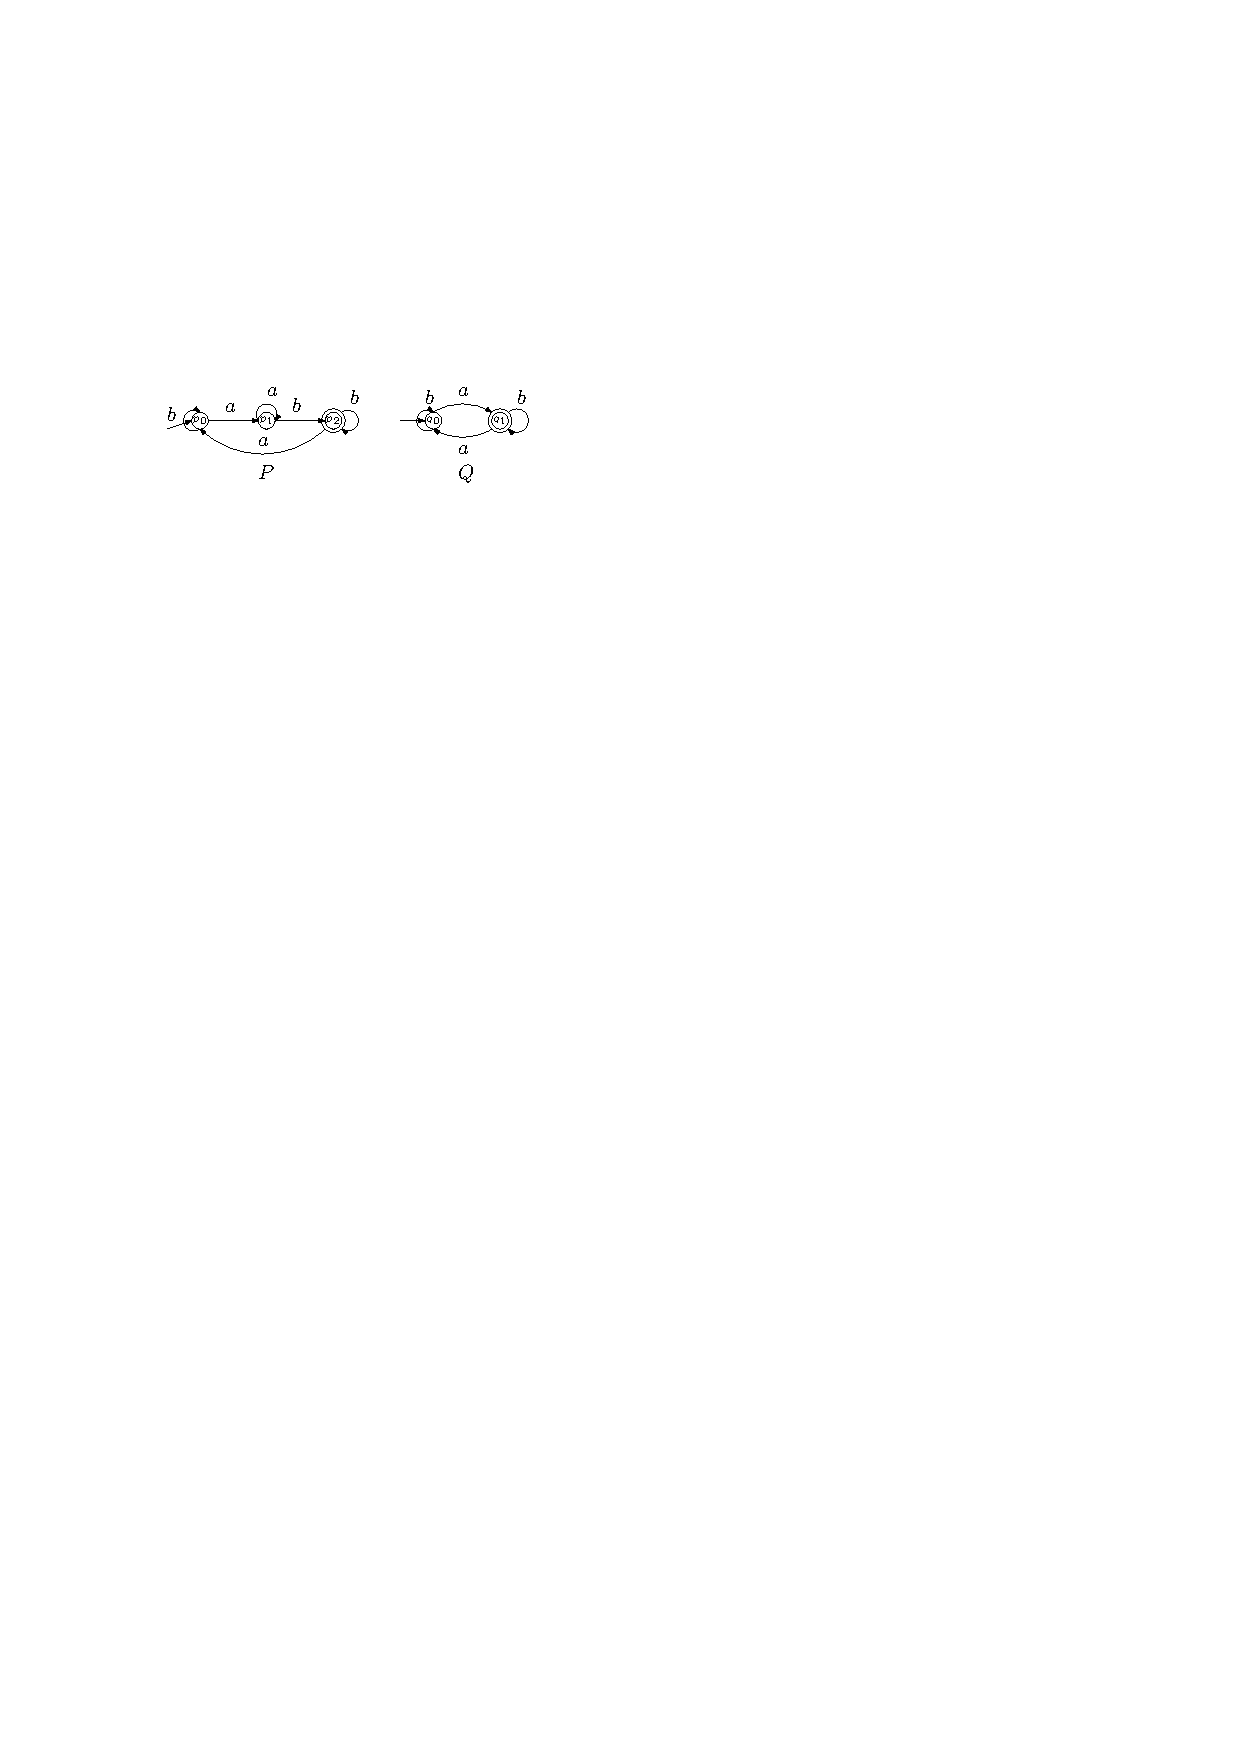
\includegraphics[width=60mm]{example_1.pdf}
\end{center}
%\vspace{-0.1in}
\caption{{\em Individual automatons}} \label{fig1}
\end{figure}

 \begin{figure}
\begin{center}
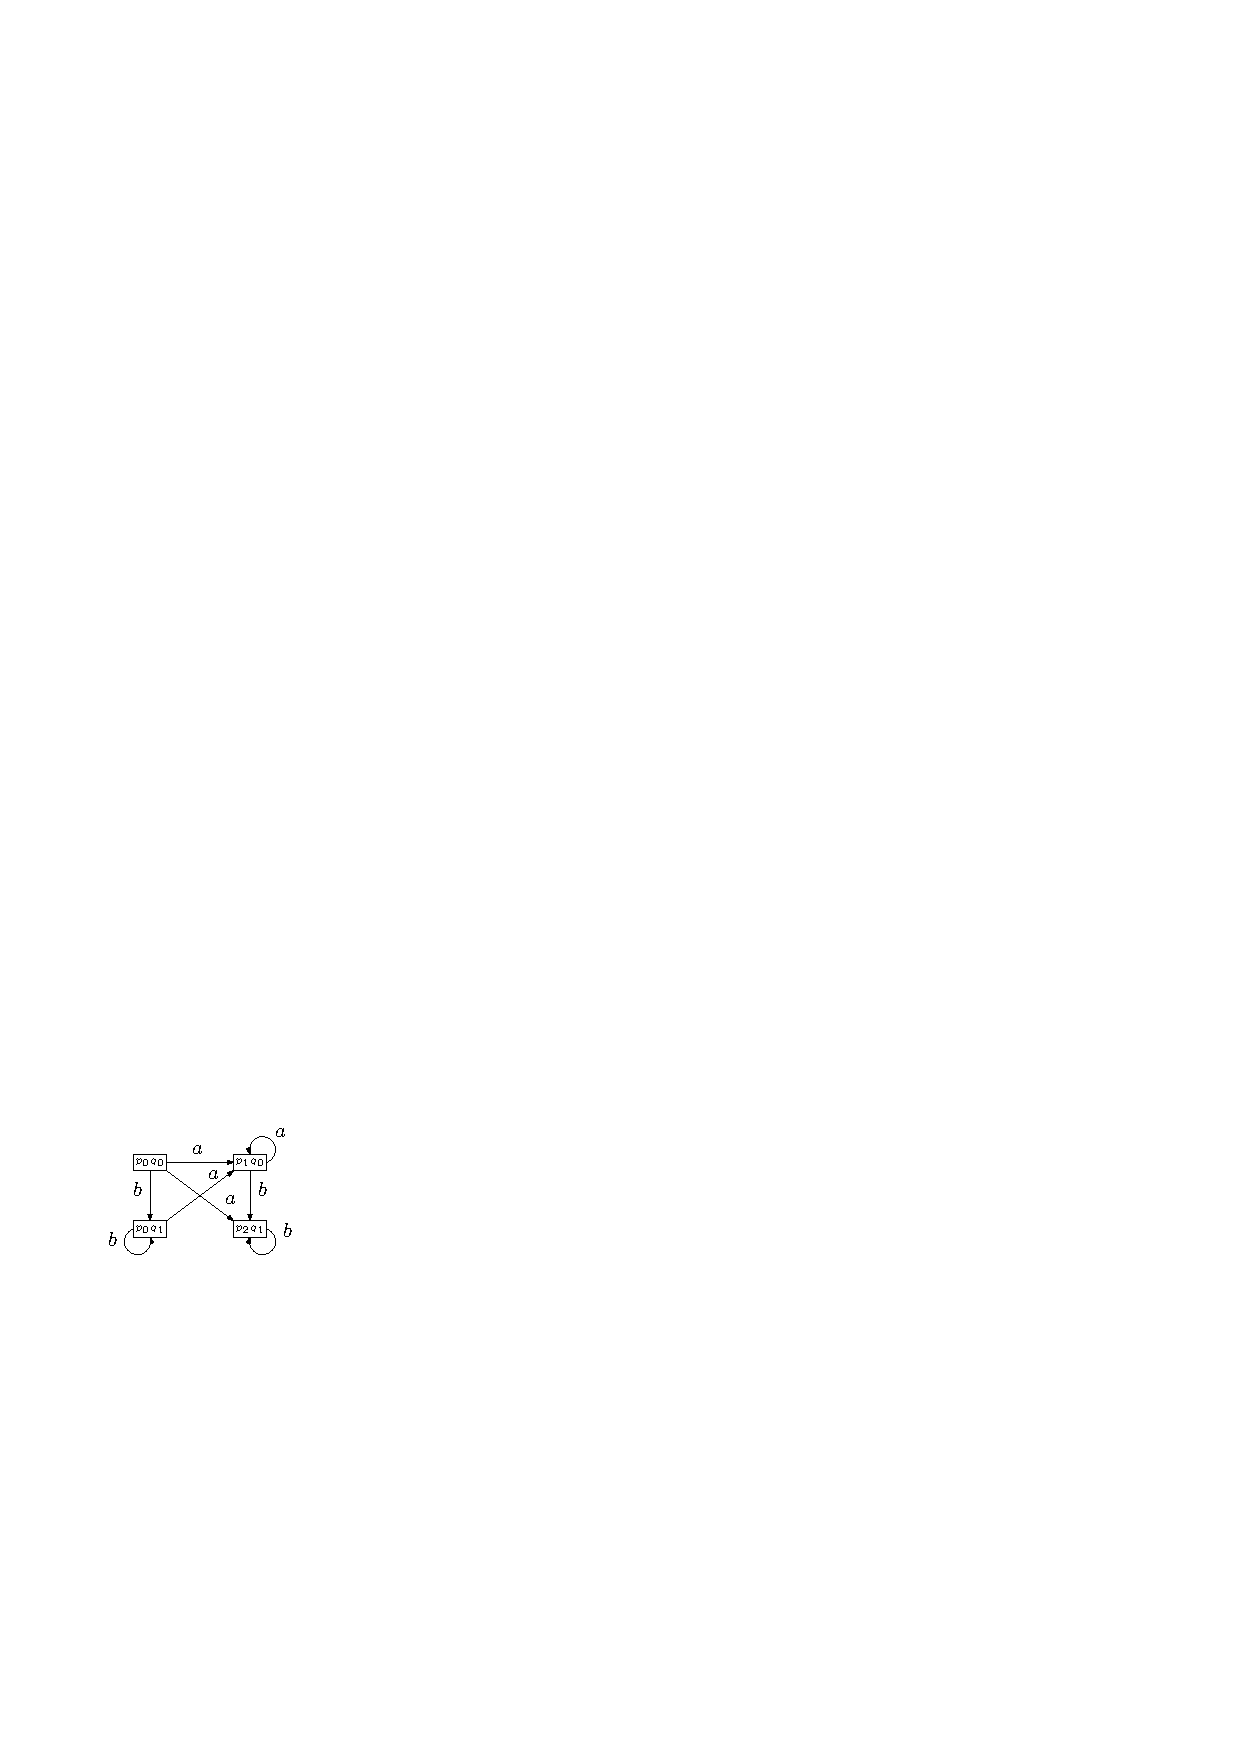
\includegraphics[width=50mm]{product.pdf}
\end{center}
%\vspace{-0.1in}
\caption{{\em Intersection of the input automata}}
\label{product}
\end{figure}
 
~\\
\noindent
Intersection of B\"{u}chi automatons require a special handling to model the infinitary acceptance condition on top of the classical product construction of finite automatons. We can see in Fig~\ref{product} that the states do not contain the tuple $<p_2,q_0>$, the set of final states
 from both the automata. In
 the following steps, we modify the product construction to include accepting states from
 both the automata. The resulting intersection automata ensures that accepting states of both the automatons are visited  infinitely often. From the set of states of each individual automaton, where each state is reachable from the 
 start state, we make three copies of the product automata. In general, for $n$ such automatons, $n$+$1$ copies are made.
 Each copy has a flag with the states, as shown in Fig\ref{fig:copy}. The flags associated with 
 the states are waiting to see the acceptance of the automaton.
In Fig \ref{fig:copy}, flag $1$ is waiting to see the acceptance state of P, flag $2$ is waiting to see
the acceptance state of Q, and states with flag $3$ signify that the track has traversed all the accepting states
of both the automatons. Starting from the first copy, the transitions are made according to the product automaton.
 A transition goes to the next flag if it gets the final state of one automaton. In general, for an automaton state associated with this flag in the product, if the acceptance condition of an automaton is obtained, the transition goes to the next copy, otherwise it remains within the transitions on its own states, as shown in  Fig\ref{transition}. When it reaches the last copy, it has traversed the accepting state of
 each individual automaton. The red cycle in Fig~\ref{transition} shows one such cycle. After reaching the last state, it goes to the first state. In the resulting automaton, a cycle is accepted, when it passes through the last copy
 of the product automaton, that signifies the run of the cycle traverses the accepting states of each automaton infinitely often. The remaining cycles, which do not pass through the last copy, are not accepted. We thus augment the classical product construction for finite automatons to model our infinitary acceptance requirement.
 
  \begin{figure}
\begin{center}
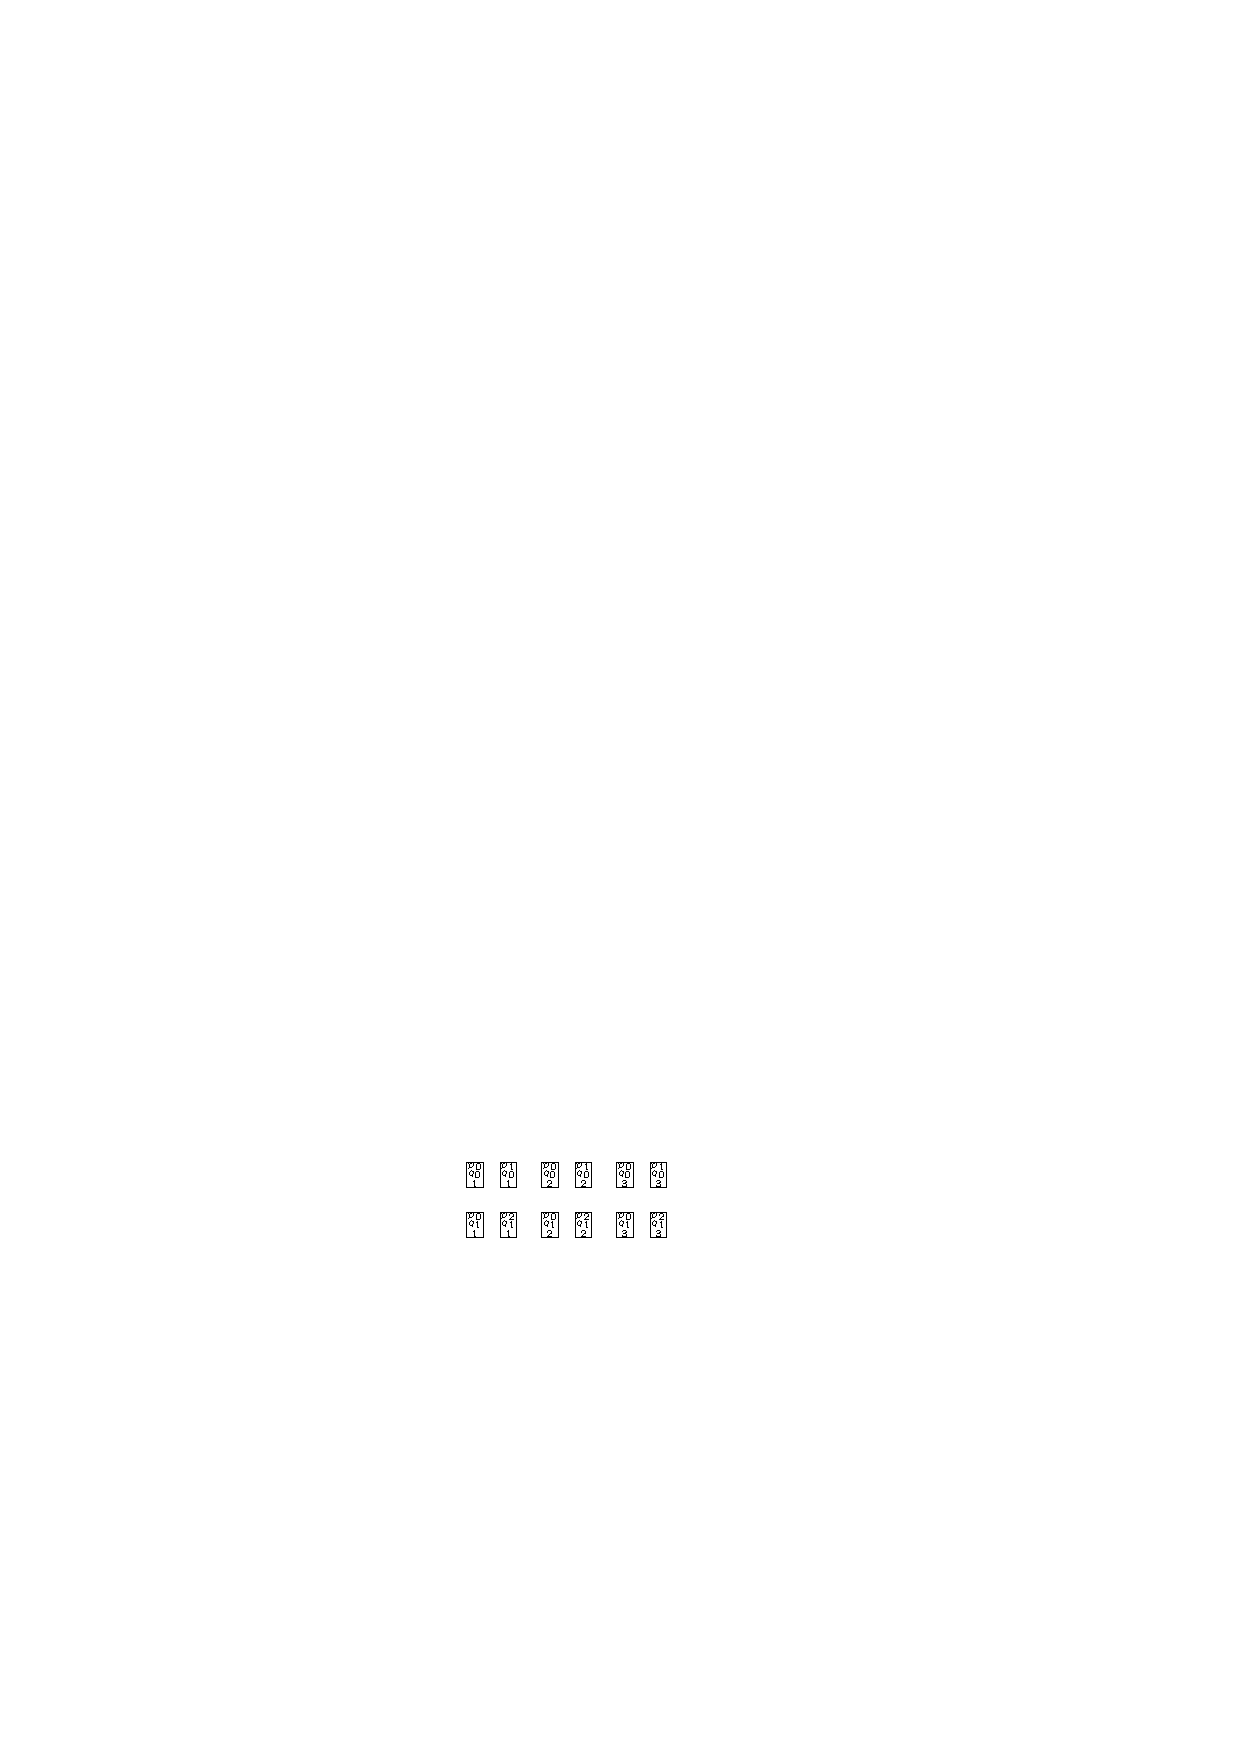
\includegraphics[width=50mm]{state_copy.pdf}
\end{center}
%\vspace{-0.1in}
\caption{{\em Product automata construction with flags}}
\label{fig:copy}
\end{figure}

 
 \begin{figure}
\begin{center}
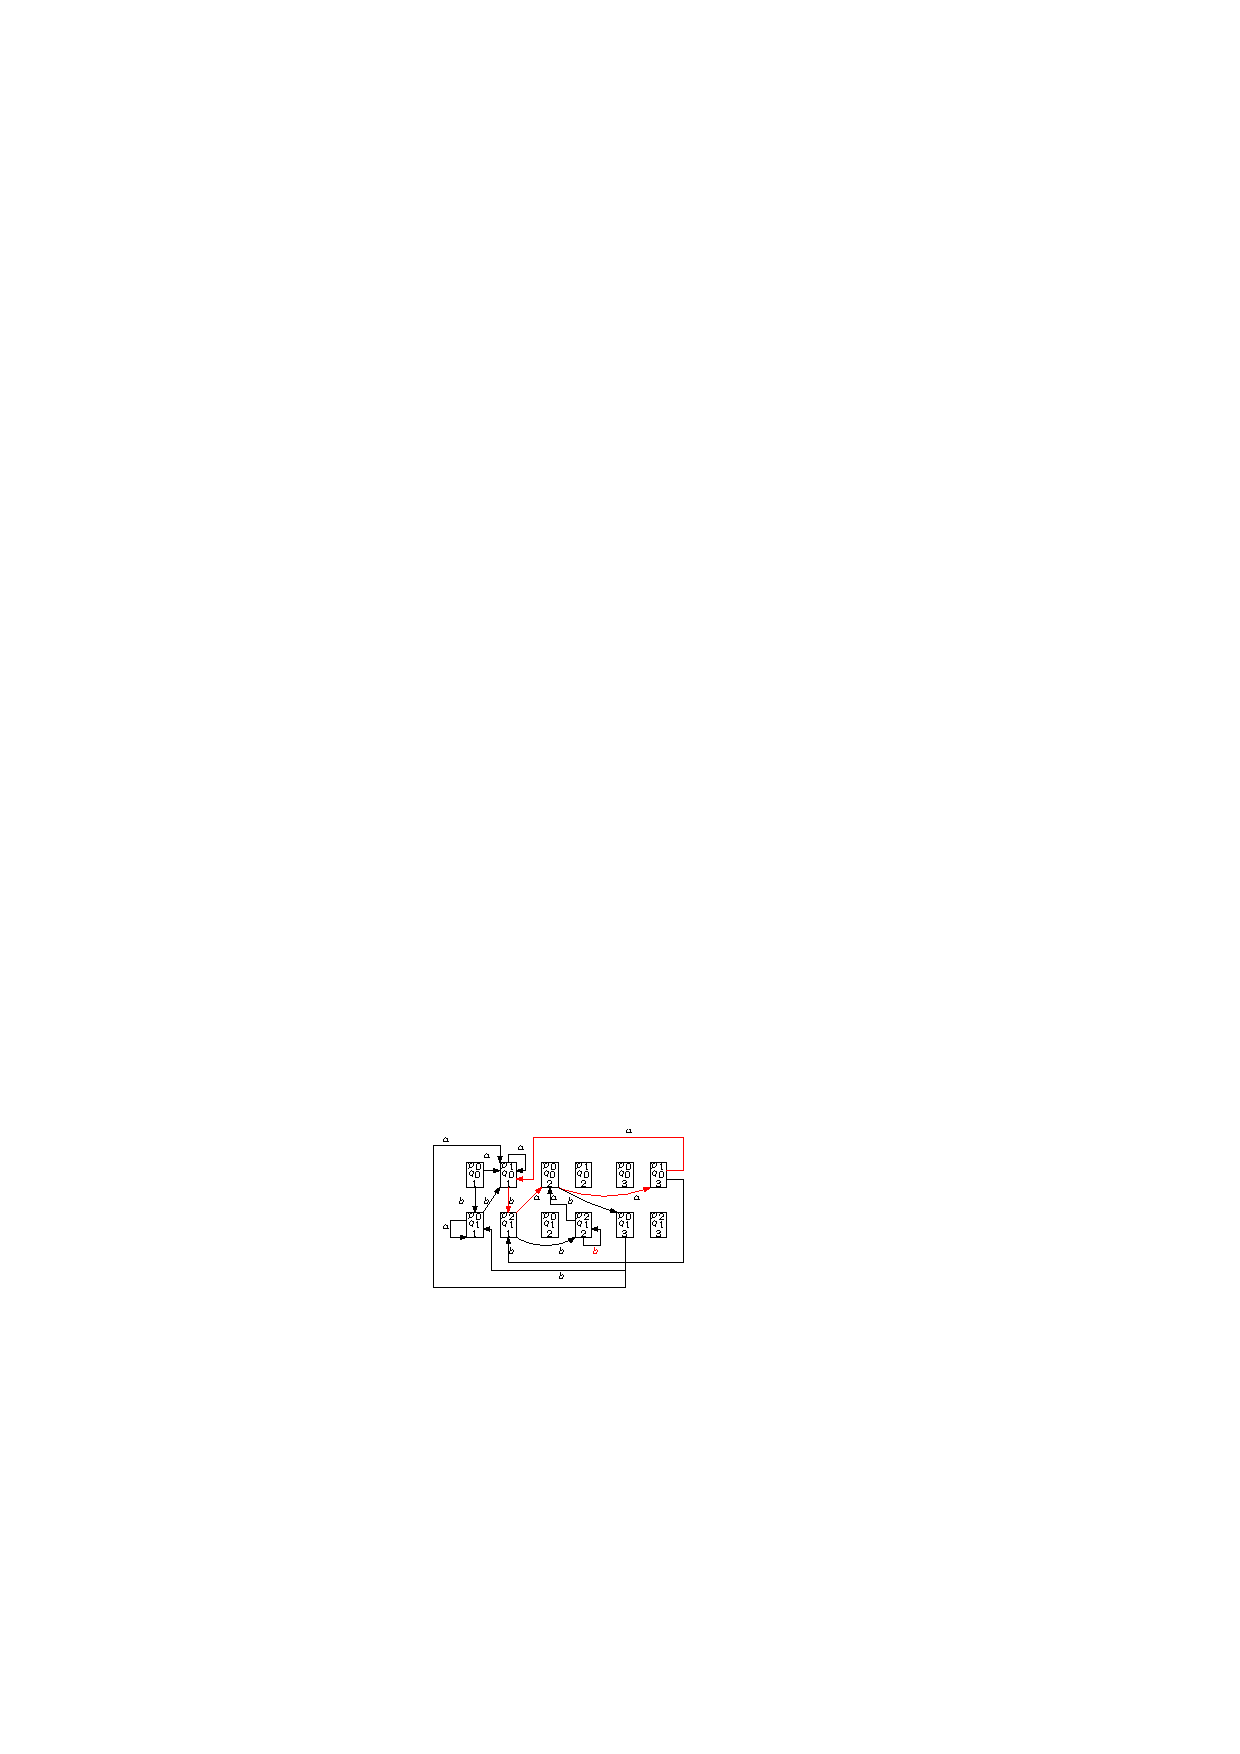
\includegraphics[width=50mm]{state_copy_transition.pdf}
\end{center}
%\vspace{-0.1in}
\caption{{\em Intersection of the input automata}}
\label{transition}
\end{figure}

\begin{figure}
\begin{center}
%\includegraphics[width=50mm, height=75mm]{algorithn.pdf}
\end{center}
%\vspace{-0.1in}
%\caption{{\em Flow chart of our idea}}
\label{fig:Algorithm}
\end{figure}

\subsection{Verifying the scheduling objective}
\noindent
Once the intersection automaton is constructed, the task of looking for cycles starting from the initial states is carried out. Cycle detection algorithms are standard in literature~\cite{Clarke:2000:MC:332656} and we implement the same for this work as well. Once a cycle is found, we traverse the cycle (every cycle is bound to contain a finite number of states) and check if each control loop is represented inside it. If not, we proceed to the next cycle and carry out the same check. If all cycles are exhausted and we do not encounter any one which meets our scheduling objective, we conclude that the schedulability requirement is not met. This step is thus quite straightforward. Consider the example given in Figure~\ref{transition}. It can be seen that there are multiple cycles in the intersection automata, some of which do not contain one representative accepting state from each control loop (e.g. $<p0,q0,1> \rightarrow <p1,q0,1> \rightarrow <p0,q1,1> \ldots$). Thus it is necessary to examine each cycle to check for existence of at least one accepting state from each control loop, which is the main idea behind the notion of schedulability we adopt here. 

\subsection{Schedulability violation attack detection}
\noindent
As the system is monitored over time, newer structures of the control loops emerge and we perform the same computation steps outlined above on the modified structures to check if it remains schedulable even in the presence of the modifications. Our mechanism can thus be used as a continuous monitor to safe-guard against intermittent control attacks. 

~\\
\noindent
At this onset, we would like to admit that our framework can point out replacement attacks only if schedulability is lost. Once the intersection is computed, we may have 3 different possibilities if schedulability is lost. Assuming that the system was schedulable earlier, we may conclude the system has been attacked if any of the following possibilities are detected. Firstly, we may have an empty intersection automaton now. As a second possibility, the product may still be non-empty but a cycle may not be reachable. Finally, a cycle may be found but it may not contain representative tasks from each control loop. All these are indicators of schedulability loss according to our analysis method and we conclude that a replacement attack is carried out. However if the system still remains schedulable according to our scheduling objective, our framework is unable to flag the attack, even if a replacement has been carried out.
\section{Toolflow} \label{sec5}
\noindent
We have built an end-to-end tool in Python for code replacement attack detection.
The tool takes in a set of control loop descriptions, computes their intersection and 
implements the cycle detection step. The tool has been applied to a number of small 
examples of synthetic control applications and their variants. The time taken for
the tool to run on a QuadCore Intel machine is in the order of milliseconds, and the
peak memory consumption is of the order of Kilobytes. Due to the lack of standard open
source benchmarks in this domain, we have not been yet able to check the performance of
our tool on more non-trivial benchmarks. 
% % % An overview of our tool is depicted in Fig \ref{tool_algorithm}.
% % % 
% % % \begin{figure}
% % % \begin{center}
% % % 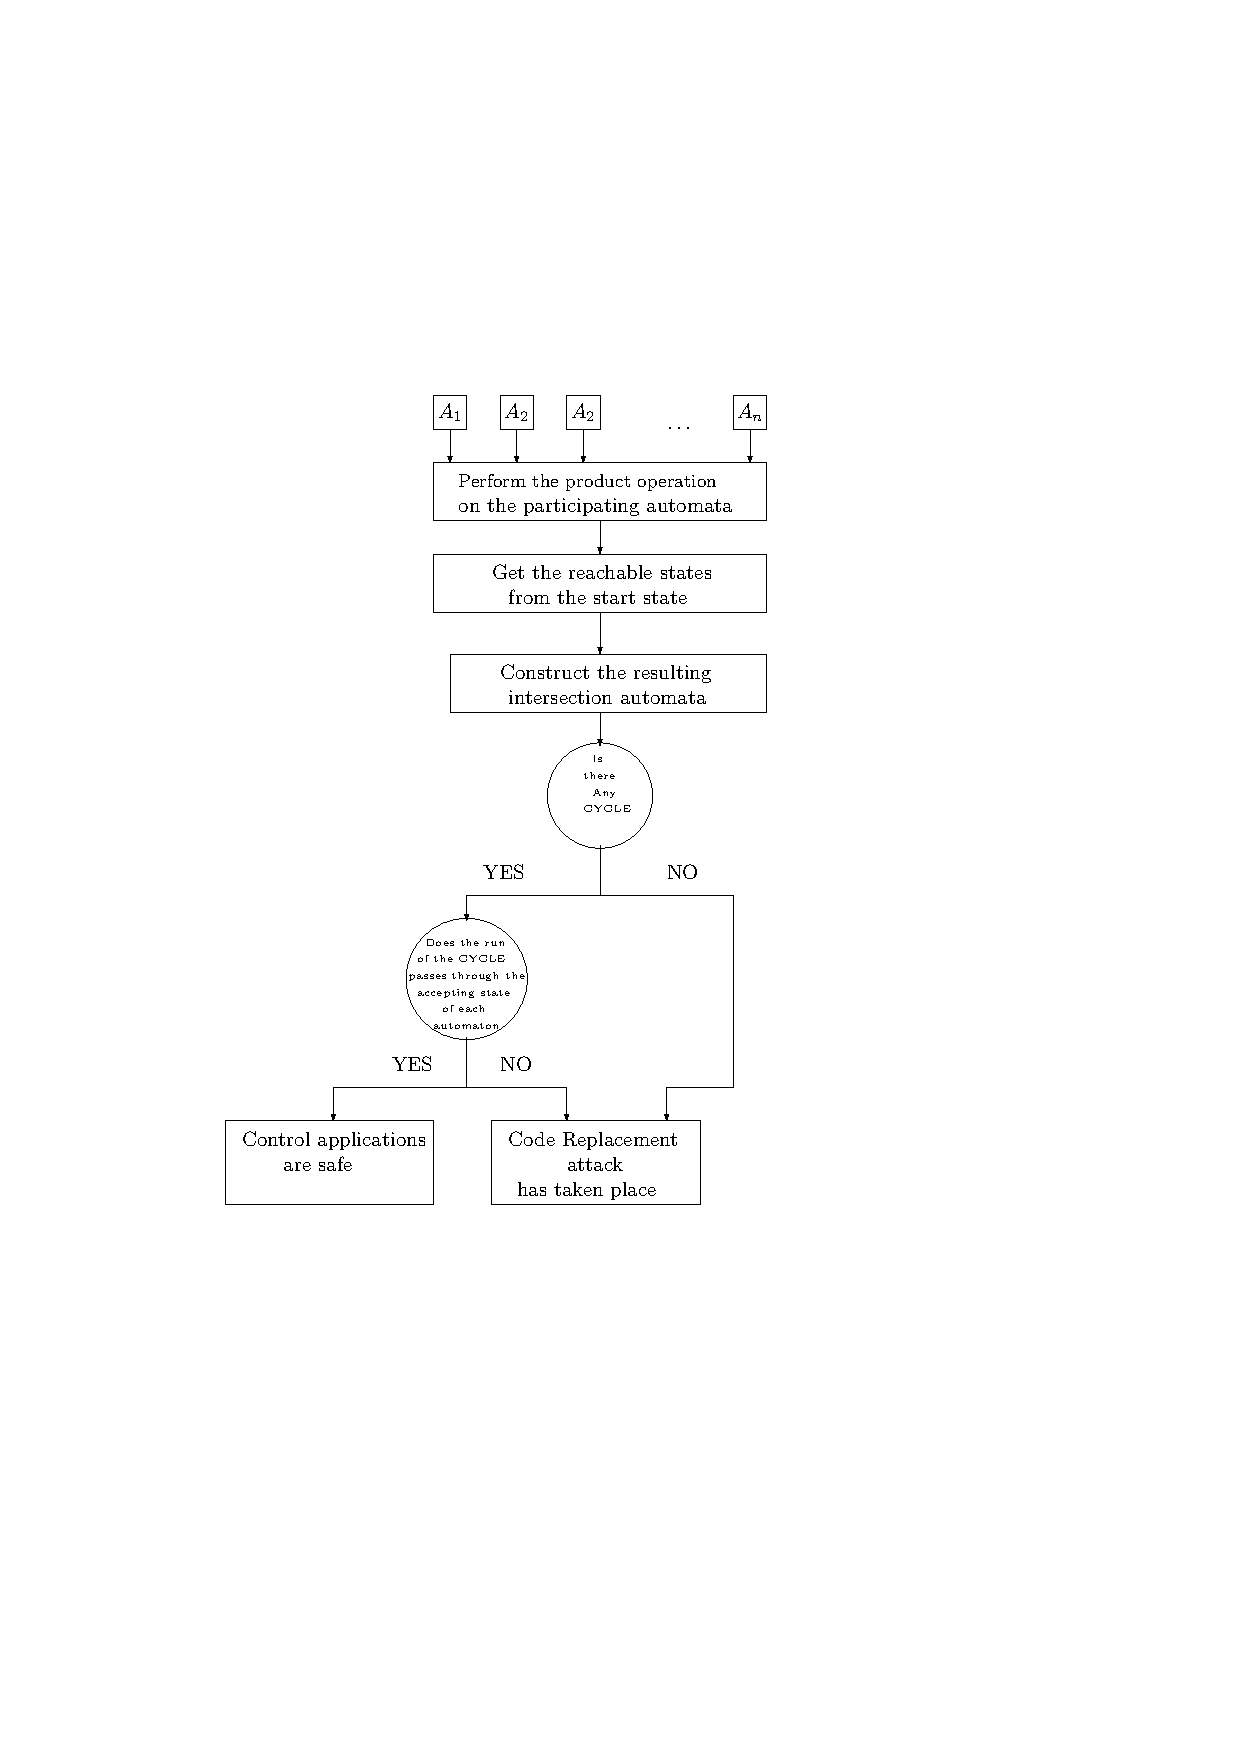
\includegraphics[width=50mm]{algorithm.pdf}
% % % \end{center}
% % % %\vspace{-0.1in}
% % % \caption{{\em The Tool flow}}
% % % \label{tool_algorithm}
% % % \end{figure}

%\input{experiment}
\section{Conclusion and Future Work} \label{sec7}
\noindent
In this work, we present an early foundation of a framework for schedulability attack detection for cyber-physical systems. We adopt standard techniques to build an automata-based control analysis foundation. We have built an end-to-end tool that implements the proposed ideas.  We are currently examining the applications of other infinitary acceptance conditions (e.g. Rabin, Muller) in this domain, with respect to their ability to detect different attack scenarios. Additionally, we are also exploring new algorithms for intersection automaton construction that might prove helpful as the number of control loops grow. We believe that our initial results will open up more interesting avenues in this research.

\bibliographystyle{IEEEtran}
{\small
\nocite{*}
\bibliography{references}
}
%\bibliographystyle{abbrv}
%\bibliography{main}
\end{document}
